
\section{Diffraction}

Diffraction is the spreading out of waves as they pass through apertures or around obstacles (i.e. any situation when they don't travel in straight lines).  The extent of the diffraction depends on the scale of the apparatus; diffraction effects only become noticable then when this scale is similar to or less than the wavelength involved.

This explains why we cannot see around corners: the wavelength of visible light is of the order of \SI{e-7}{m}, which is so small that no diffraction is seen with obstacles of normal size.  A typical Young's double slits apparatus is about a metre long (about 10 million times the wavelength of light) and the slits themselves are about a thousand wavelengths across.  Diffraction effects are observable on this scale, but only with care.

In contrast, on a human scale we are very familiar with the diffraction effects of sound, being able to hear it round wide openings like doorways as the wavelength is comparable with the width of the opening (middle C has a frequency of about \SI{262}{Hz}, meaning its wavelength will be \SI{1.3}{m}).  Generally, diffraction increases with longer wavelength---things `seem smaller' to the wave---and for this reason, high pitched sounds can be more easily heard from around corners and through doorways than lower pitches.\footnote{When vibrations from sound waves are transmitted through walls, the converse is true: lower frequencies are transmitted better.}

\subsection{Historical importance}

In 1665, Grimaldi observed that the shadow of a thin wire in a light beam was much broader than he expected, and invented the word `diffractio' to describe the bending of the light (from the Italian meaning `break' or `snap').  Although Newton repeated this experiment, its true significance---that in certain circumstances, light can bend round corners---had to wait more than a century to be recognized, when Huygens' wave theory of light had once again gained acceptance.  Another example was provided by Poisson, who worked out mathematically that the superposition of the waves from the edge of a small circular disk ought to produce a bright spot in the center of its shadow.  He thought this impossible, but when experiment confirmed his prediction, he became a supporter of the wave theory of light.

\subsection{Diffraction at a single slit}

Suppose parallel wavefronts are diffracted at a narrow opening or slit.  This is called \emph{Fraunhofer diffraction}.\footnote{The diffraction of circular wavefronts from a near object is called \emph{Fresnel diffraction}, which we shall not study.}  This effect is easily demonstrated for water waves using a ripple tank, which will show the spreading of the wavefronts beyond the opening, and also the dependence on the wavelength and size of opening.

\vspace*{1em}

%pictures of wave tank??
\begin{minipage}{0.45\textwidth}
\includegraphics[width=0.8\textwidth]{img/waterdiffraction1.jpg}
\end{minipage}
\begin{minipage}{0.45\textwidth}
\includegraphics[width=0.8\textwidth]{img/waterdiffraction2.jpg}
\end{minipage}\\
{\scriptsize Images: ANDREW LAMBERT PHOTOGRAPHY/SCIENCE PHOTO LIBRARY}

\vspace*{1em}

Light can also be shown to diffract at a single slit.  The single slit is illuminated with a coherent beam of light (from a laser) and the section of beam which passes through the slit diffracts to form the characteristic intensity pattern shown.  The maximum brightness of the pattern occurs immediately ahead of the slit and decreases to each side.  Not only is there a central intense spread, but subsidiary maxima and minima can also be seen on both sides (these are not easily observed for water waves).


\noindent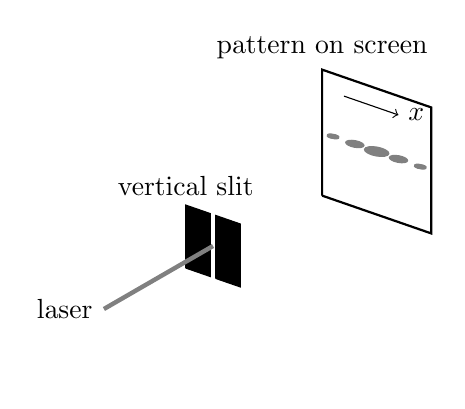
\begin{tikzpicture}[x={(0.866cm,-0.3cm)}, y={(0.866cm,0.5cm)}, z={(0cm,1cm)}, scale=0.8]
%slit:
\draw[fill] (-0.5,2,-0.5)-- (-0.05,2,-0.5)-- (-0.05,2,0.5)-- (-0.5,2,0.5)node[above]{vertical slit}--(-0.5,2,-0.5);
\draw[fill] (0.05,2,-0.5)-- (0.5,2,-0.5)-- (0.5,2,0.5)-- (0.05,2,0.5)--(0.05,2,-0.5);
%beam:
\draw[ultra thick,gray] (0,0,0)node[left,black]{laser} -- (0,2,0);
%screen:
\draw[thick] (-1,5,-1)-- (1,5,-1)-- (1,5,1)-- (-1,5,1)node[above]{pattern on screen}--(-1,5,-1);
%axis:
\draw[->] (-0.6,5,0.7) --(0.4,5,0.7)node[right]{$x$};
%diffraction pattern
\draw[fill,gray] (0,5,0) ellipse (0.2 and 0.1);
\draw[fill,gray] (0.4,5,0) ellipse (0.15 and 0.075);
\draw[fill,gray] (-0.4,5,0) ellipse (0.15 and 0.075);
\draw[fill,gray] (0.8,5,0) ellipse (0.1 and 0.05);
\draw[fill,gray] (-0.8,5,0) ellipse (0.1 and 0.05);
\node at (0,0,-1) {};
\end{tikzpicture}\hspace{0em}
\begin{tikzpicture}[scale=0.5]
\draw[->] (-5.5,0)--(5.5,0)node[right]{$x$};
\draw plot[smooth,domain=-5:5,samples=100] (\x, {0.5*(sin(\x r * 3.14159 / 1)/\x)^2});
\draw[->] (0,0)--(0,5.5)node[above]{Intensity};
\node (pattern) at (0,-1.6) {\includegraphics[scale=0.8]{img/singleslitpatterngreen2.jpg}};
\node (label) at (0,-3.3) {\tiny Image: EDWARD KINSMAN/SCIENCE PHOTO LIBRARY};
\end{tikzpicture}

The central broad maximum is twice as wide as all the other bright bands, and the minima going outwards from this are evenly spaced in terms of angular displacement.\footnote{The angular positions $\theta_{n}$ of successive minima are given by $d\sin\theta=n\lambda$, where $d$ is the slit width, $\lambda$ is the wavelength of the light, and $n$ is the order of the minimum.}  However, the intensities of the illuminated bands between the minima fall away very markedly, all being much less intense than the larger central band, and so a dark room and good equipment is needed to see more than two or three bands on each side of the maximum.  

With a narrower slit (or equivalently a longer wavelength of light) the light spreads out more as diffraction is more pronounced, and this is why the light is seen to spread out in the direction of the smallest dimension of the slit, i.e.\ a horizontal pattern of bands is seen for a vertical slit.  A narrower slit also allows less wave energy to pass through it, and hence the brightness at any point on the screen is reduced.

%\subsubsection{Why are there minima in the single slit diffraction pattern?}

%[{\em non-examinable}] At first sight it is surprising that there are repeated maxmima and minima from diffraction from a single slit, so this aspect of the pattern requires further thought and explanation.  A full mathematical treatment of the diffraction pattern is well beyond the scope of these notes,\footnote{For such a treatment, see for example {\em Optics} by  Eugene Hecht, published by Addison Wesley.} but it is possible to give an idea of how the subsidiary maxima and minima come about.


%\begin{tikzpicture}
%\draw[ultra thick] (0,0.2)--(0,2);
%\draw[ultra thick] (0,-0.2)--(0,-2);
%\foreach \i {1,...,5}{
%\draw (-1,\i)--(0,\i);
%}
%\end{tikzpicture}\hspace{2em}